\documentclass [listof=totoc,bibliography=totoc,english,a4paper,titlepage] {scrartcl}

\usepackage[english]{babel}
\usepackage{setspace}
\usepackage[paper=a4paper]{geometry}
\usepackage[utf8]{inputenc}
\usepackage{amsmath}
\usepackage{dsfont}
\usepackage{graphicx}
\usepackage{textcomp}
\usepackage{subfigure}
\usepackage{esvect}
\usepackage{pstricks}
\usepackage{floatflt}
\usepackage{SIunits}
\usepackage{amsopn}
\usepackage[percent]{overpic}

\setlength{\parskip}{6pt}
\setlength{\parindent}{0pt}

\onehalfspacing

\renewcommand{\thefigure}{\arabic{section}.\arabic{figure}}
\makeatletter \@addtoreset{figure}{section} \makeatother
\renewcommand{\thetable}{\arabic{section}.\arabic{table}}
\makeatletter \@addtoreset{table}{section} \makeatother
\renewcommand{\theequation}{\arabic{section}.\arabic{equation}}
\makeatletter \@addtoreset{equation}{section} \makeatother

\let\oldbibitem=\bibitem
\renewcommand{\bibitem}{%
\filbreak
\oldbibitem
}

\newenvironment{changemargin}[2]{%
  \begin{list}{}{%
    \setlength{\topsep}{0pt}%
    \setlength{\leftmargin}{#1}%
    \setlength{\rightmargin}{#2}%
    \setlength{\listparindent}{\parindent}%
    \setlength{\itemindent}{\parindent}%
    \setlength{\parsep}{\parskip}%
  }%
  \item[]}{\end{list}}


\newenvironment{mylisting}
{\begin{list}{}{\setlength{\leftmargin}{1em}}\item\scriptsize\bfseries}
{\end{list}}

\DeclareMathOperator{\grad}{grad}

\makeatletter
\let\divsymb\div              % make \IEEEendproof do same as \endproof
\let\div\@undefined                  % undefine \endproof
\makeatother

\DeclareMathOperator{\div}{div}

\begin{document}

%
%% Titelblatt
%%


\thispagestyle{empty} %% ohne Kopf- und Fusszeile, Seitennummer etc.

%% eigene Umgebung schaffen -> minipage
\begin{titlepage}     %% Anfang Sichtfenster

	\sffamily
	\begin{center}
		\vspace{1cm}
		
		\large{\textbf{Rheinisch-Westfälische Technische Hochschule Aachen\\Institut für Bildsame Formgebung}}
		
		\vspace{20mm}
				
		\Large{\textbf{Title bla blubb \\}}
		%\vspace{-0.35cm}
		\Large{\textbf{blubb bla}}
		
		\vspace{2cm}
		

		
		\LARGE{\textbf{Hauptseminar}} \\
		
		\vspace{1.5cm}
		
		\large{Paul Hibbe, B.Sc. \\ Matthias Nick, B.Sc.}\\
		
		\vspace{3cm}
		\end{center}
		
	%\large{Thema:\hspace{0.5cm}	Vergleich unterschiedlicher Dehnungsmessmethoden im quasistatischen Zugversuch\\ \hspace{2.0cm}}

	
\begin{center}
\large{Durchgeführt in der Abteilung Werkstoffmodellierung \\ im WS 2013/14}
\end{center}

\vspace{3cm}
\begin{tabbing}
\hspace*{3cm}\=\hspace{2cm}\=\kill
Betreuer: \>Univ. Prof. Dr.-Ing. Gerhard Hirt\\
          \>Dipl.-Ing. Thomas Henke\\
          \>Stephan Hojda, M.Sc.
\end{tabbing}
\end{titlepage} %% Ende Sichtfenster

\tableofcontents

\pagebreak

\section{Einleitung}

In der Fertigung von Prototypen und Kleinserien ist die Anwendung traditioneller Blechumformverfahren wie des Tiefziehens oder des Streckziehens aufgrund der Notwendigkeit von hochfesten Werkzeugen und Maschinen, die hohe Kräfte aufbringen können, sowohl kosten- als auch zeitintensiv. Ein Prozess, der diese Beschränkungen umgeht, ist die inkrementelle Blechumformung (IBU), welche mit einem universellen Werkzeug, das Blech inkrementell umformt. Für die IBU ergeben sich jedoch einige Prozessgrenzen. Neben der langen Dauer des Prozesses und seiner schlechten Abbildbarkeit in Simulationen sind dies insbesondere die Neigung zu Ausdünnung, Einschnürung und schließlich Riss des Blechs bei hohen Wandwinkeln sowie die schlechte Geometriegenauigkeit. \cite{dissbambach,dissames}\par

Das Problem der Geometriegenauigkeit zeigt sich besonders bei schwerumformbaren Werkstoffen wie dem in der Luftfahrt oft verwendeten TiAl6V4. Dieses besitzt neben einem niedrigen Elastizitätsmodul auch eine hohe Fließgrenze, so dass ein großer elastischer Anteil an der Formänderung besteht. Dies wiederum führt zur Rückfederung des Werkstücks nach dem Umformen. Weiterhin ist das Umformvermögen von TiAl6V4 bei Raumtemperatur nur gering. Zur Überwindung dieser Prozessgrenzen wurden bereits Versuche unternommen, die Fließspannung des umzuformenden Blech durch Erwärmung zu senken. Neben der Erwärmung des gesamten Bleches während des Prozesses ist es möglich, den Werkstoff gezielt in der Umformzone zu erwärmen. Dies kann konduktiv oder mit Laserstrahlung erfolgen. \cite{hybridisf,diplbailly}\par

Zur laserunterstützten inkrementellen Blechumformung ist bereits eine Optik entwickelt worden, die es ermöglicht, den Laserbrennfleck um das Umformwerkzeug herum zu bewegen. Ebenfalls existiert bereits ein Programm, welches auf Basis eines bestehenden NC-Pfads zu einem IBU-Prozess die notwendigen Bewegungen des Laserbrennflecks bestimmt \cite{laseraisfti}. Es ist jedoch aus thermischen und geometrischen Gründen nicht sinnvoll, den Laser dauerhaft mit der gleichen Ausgangsleistung zu betreiben. Daher ist das Thema dieser Arbeit eine Vorausberechnung der benötigten Laserleistung unter Berücksichtigung der tatsächlichen Geschwindigkeit des Laserbrennfelcks und von Wärmeleitungs- und Wärmeverlustphänomenen sowie eine theoretische Validierung des dazu entwickelten Algorithmus und das Erstellen eines Konzepts für die Einbindung in das bestehende CAX-Umfeld.
\section{Fundamentals}

\subsection{Open-die forging}
The incremental and flexible nature of open-die forging makes it suitable primarily to the manufacturing of small lot sizes or for the forming of parts that cannot be produced by other processes due to power and force limitations of these processes. Its primary use is in the preparation of cast ingots for further machining. By open-die forging, cavities from the casting process can be rectified and the needed material properties can be reached.\cite{forgcomp}

\subsection{Finite element method}
The finite element method is a method to model, beside others, continuum mechanics of solid work pieces. The work piece is separated into discrete parts, called elements, which are themselves geometrically defined by nodes. While these nodes hold coordinates as information, the elements hold temperatures, stresses etc. Using material properties such as flow curves, friction, thermal conductivity and emissivity, the system's reaction to thermal and mechanical external loads can be calculated.

Due to the non-linear nature of the resulting equation system, only very simple models can be calculated analytically while most must be approximated numerically. Besides matters of usability, the numerical approach is the most important difference between available software packages. These are spread across a wide spectrum from academic systems with large freedom for the user to easy-to-use specialized tools for certain uses.

%\section{Geometrische und thermische Grundlagen der Erwärmung mit Laser}

Zur Bestimmung der bei der Lasererwärmung eingetragenen Wärme ist die Betrachtung von zwei unterschiedlichen Teilaspekten notwendig: Zum Einen der Einfluss der Bewegungsgeschwindigkeit des Laserflecks, zum Anderen derjenige der Eigenschaften des verwendeten Werkstoffes.

\subsection{Geschwindigkeit des Laserbrennflecks}

Zur Bestimmung der Geschwindigkeit des Laserflecks wird das System in dreidimensionalen Koordinaten betrachtet. In diesen Koordinaten stellt sich die Bewegungsgeschwindigkeit $\vv{v_t}$ des Werkzeugs dar als:
\begin{equation}
 \vv{v_t} = \left(\begin{array}{c}v_{t,x}\\v_{t,y}\\0\end{array}\right)
 \label{eqn:toolvel3d}
\end{equation}

Weiterhin gilt für die Winkelgeschwindigkeit $\vv{\dot{\varphi}}$ der Bewegung des Laserflecks:
\begin{equation}
 \vv{\dot{\varphi}} = \left(\begin{array}{c}0\\0\\\dot{\varphi}\end{array}\right)
 \label{eqn:laserrotvel3d}
\end{equation}
 
Zudem ergibt sich aus der Geometrie des Aufbaus %(Abbildung \ref{img:geovel})
für den Radialvektor $\vv{r}$ mit der Entfernung $d_l$ des Laserflecks von der Rotationsachse:
\begin{equation}
\vv{r} = d_l\left(\begin{array}{c}-\sin\varphi\\\cos\varphi\\0\end{array}\right)
\label{eqn:radvec3d}
\end{equation}

% \begin{figure}[htbp]
%  \centering
%  \begin{pspicture}(8,5)
%   \psline{->}(4,1)(8,1)
%   \rput(8,0.6){x}
%   \psline{->}(4,1)(4,5)
%   \rput(3.6,5){y}
%   {
%    \SpecialCoor
%    \rput(4,1)
%    {
%     \psline(3.5;90)(0,0)(3.5;120)
%     \psarc{->}(0,0){3}{90}{120}
%     \rput[br](3.1;105){$\varphi$}
%    }
%   }
%  \end{pspicture}
%  \caption{Geometrie der Anordnung des Laserflecks}
%  \label{img:geovel}
% \end{figure}

Für den Geschwindigkeitsvektor $\vv{v_l}$ des Laserflecks gilt nun:
\begin{equation}
 \vv{v_l} = \vv{v_t} + \vv{\dot{\varphi}} \times \vv{r}
 \label{eqn:dotvelcomp}
\end{equation}

Einsetzen von Gleichungen \ref{eqn:toolvel3d}, \ref{eqn:laserrotvel3d} und \ref{eqn:radvec3d} in Gleichung \ref{eqn:dotvelcomp} und Umformen ergibt:
\begin{equation}
 \vv{v_l} = \left(\begin{array}{c}v_{t,x}\\v_{t,y}\\0\end{array}\right) - d_l\; \dot{\varphi} \left(\begin{array}{c}\cos\varphi\\\sin\varphi\\0\end{array}\right)
 \label{eqn:dotvelfin3d}
\end{equation}

Da das Problem im Prinzip zweidimensional ist und in Gleichung \ref{eqn:dotvelfin3d} die dritte Komponente immer null ist, liegt es nahe, die Gleichung in zwei Dimensionen darzustellen:
\begin{equation}
 \vv{v_l} = \left(\begin{array}{c}v_{t,x}\\v_{t,y}\end{array}\right) - d_l\; \dot{\varphi} \left(\begin{array}{c}\cos\varphi\\\sin\varphi\end{array}\right)
 \label{eqn:dotvelfin2d}
\end{equation}

Interessant ist jedoch nur der Betrag der Geschwindigkeit des Laserflecks, welcher sich wie folgt bestimmt:
\begin{equation}
 v_l = \left|\vv{v_l}\right| = \sqrt{\left(v_{t,x} - d_l\dot\varphi\cos\varphi\right)^2 + \left(v_{t,y} - d_l\dot\varphi\sin\varphi\right)^2}
 \label{eqn:dotvelabs}
\end{equation}

\label{sec:geotheory}

\subsection{Durch Laserstrahlung eingetragene Wärme}

Die Strahlungsenergie des Lasers wird im Blech in innere Energie in Form von Wärme umgewandelt. Laut \cite{atkins} gilt für die infinitesimale Temperaturänderung $dT$ durch die Änderung der inneren Energie $dU$ bei der spezifischen Wärmekapazität $C_{V,s}$ und konstantem Volumen:
\begin{equation}
  dT = \frac{dU}{mC_{V,s}}
  \label{eqn:specificheat}
\end{equation}

wobei $m$ die Masse des erwärmten Stoffes darstellt. Auf einem Teil eines Bleches der Dicke $d_s$, welches die Länge $l_e$ und die Breite $b_e$ besitzt (s. Abbildung \ref{img:element}), bestimmt sich die Masse über die Dichte $\rho$ zu:

\begin{equation}
 m = \rho V = \rho d_s l_e b_e
 \label{eqn:massgeometry}
\end{equation}

\begin{figure}[!btp]
 \centering
 \includegraphics[width=0.8\textwidth]{images/element}
 \caption{Skizze eines Volumenelements zur Bestimmung der Wärmekapazität}
 \label{img:element}
\end{figure}

Mit dieser Beziehung und Gleichung \ref{eqn:specificheat} ergibt sich für die Änderung der Temperatur:
\begin{equation}
  dT = \frac{dU}{\rho d_s l_e b_eC_{V,s}}
  \label{eqn:tempgeometry}
\end{equation}

Weiterhin ist die Leistung $P$ definiert als die Änderung der Energie mit der Zeit, also gilt:
\begin{equation}
  P = \frac{dU}{dt}\;\;\Leftrightarrow\;\; dU = Pdt
  \label{eqn:definitionpower}
\end{equation}

Laut \cite{laserheating} gilt für die absorbierte Leistung $P_a$:
\begin{equation}
  P_a = \alpha P_g
  \label{eqn:absorptivity}
\end{equation}

mit dem Absorptionsgrad $\alpha$ und der gesamten eingestrahlten Leistung $P_g$. Diese wiederum lässt sich mit $b_e'$, der Breite des vom Laserflecks getroffenen Teil des betrachteten Blechteils, sowie der Breite des gesamten Laserflecks $b_l$ und der Laserleistung $P_l$ abschätzen zu:
\begin{equation}
  P_g = \frac{b_e'}{b_l}P_l
  \label{eqn:powerfrac}
\end{equation}

Hierbei wird davon ausgegangen, dass die Laserleistung über die gesamte Breite des Laserflecks gleichverteilt ist. Einsetzen von Gleichung \ref{eqn:powerfrac} in Gleichung \ref{eqn:absorptivity} und dieser in \ref{eqn:definitionpower} ergibt:
\begin{equation}
  dU = \frac{b_e'}{b_l}\alpha P_l dt
  \label{eqn:energyofpower}
\end{equation} 

Dies wiederum ergibt mit Gleichung \ref{eqn:tempgeometry} einen Zusammenhang zwischen der Temperaturänderung und der Laserleistung:
\begin{equation}
  dT = \frac{1}{\rho d_s l_e b_eC_{V,s}} \frac{b_e'}{b_l}\alpha P_l dt = C \frac{b_e'}{b_l}\alpha P_l dt
  \label{eqn:dTofdt}
\end{equation}

Hierbei ist $C = \frac{1}{\rho d_s l_e b_eC_{V,s}}$ mit der Zeit konstant. Integrieren beider Seiten von $t'=0$ bis $t'=t$ ergibt:
\begin{equation}
  \Delta T = \int_{T(0)}^{T(t)} dT = \int_{0}^{t} C \frac{b_e'}{b_l}\alpha P_l dt' = C \frac{b_e'}{b_l} P_l \int_{0}^{t} \alpha dt'
  \label{eqn:integrationtemp}
\end{equation}

Dies ist zulässig, da laut \cite{laserheating} nur der Absorptionsgrad sich zwischen Raumtemperatur und Schmelztemperatur eines Metalls maßgeblich ändert. Dieser lässt sich mit der folgender Näherung beschreiben:

\begin{equation}
\alpha(T) = \alpha_0 + \alpha_1 T
\end{equation}

Dies würde jedoch eine Integration der rechten Seite von Gleichung \ref{eqn:integrationtemp} sehr kompliziert machen. Daher wird ein vereinfachter Absorptionsgrad $\alpha'$ eingeführt, der das Gesamtergebnis der Integration nicht beeinflusst, diese jedoch deutlich vereinfacht. Dazu lässt sich Gleichung \ref{eqn:dTofdt} umformen zu:

\begin{equation}
 \frac{\rho d_sl_eb_eC_{V,s}b_l}{b_e'}\frac{dT}{\alpha(T)} = c \frac{dT}{\alpha_0 + \alpha_1 T} = P_l dt
 \label{eqn:alphaintpreconst}
\end{equation}

wobei $c = \frac{\rho d_sl_eb_eC_{V,s}b_l}{b_e'P_l}$ als temperaturunabhängig gesehen werden kann. Integration ergibt:
\begin{equation}
  \int_{T_R}^{T_Z}c\frac{dT}{\alpha_0 + T \alpha_1} = c\frac{\ln\left(\alpha_0 T_Z + \alpha_1\right)-\ln\left(\alpha_0 T_R + \alpha_1\right)}{\alpha_1} = \Delta U = \int_0^t P_l dt'
\end{equation}

Wird nun $\alpha'$ eingeführt als 

\begin{equation}
\alpha' = \frac{\alpha_1 \Delta' T}{\ln\left(\alpha_0 T_Z + \alpha_1\right)-\ln\left(\alpha_0 T_R + \alpha_1\right)}
\label{eqn:alphas}
\end{equation}

mit $\Delta'T = T_Z-T_R$ der Differenz zwischen Zieltemperatur und Raumtemperatur, so ergibt sich, dass ein Ersetzen von $\alpha$ durch $\alpha'$ bei der Betrachtung der gesamten Temperaturdifferenz keinen Fehler einführt.

\begin{eqnarray}
  \int_{T_R}^{T_Z}c\frac{dT}{\alpha'} &=& c\int_{T_R}^{T_Z}\frac{\ln\left(\alpha_0 T_Z + \alpha_1\right)-\ln\left(\alpha_0 T_R + \alpha_1\right)}{\alpha_1 \Delta' T} dT\\\nonumber
   &= &c\frac{\ln\left(\alpha_0 T_Z + \alpha_1\right)-\ln\left(\alpha_0 T_R + \alpha_1\right)}{\alpha_1}\\
   &= &\int_{T_R}^{T_Z}c\frac{dT}{\alpha}
\end{eqnarray}

Somit kann durch diese vereinfachte Betrachtung die Entwicklung der Temperatur zwischen Raumtemperatur und Zieltemperatur nicht vorhergesagt werden. Dies führt in diesem Fall jedoch nicht zu Problemen, da einzig die zuzuführende Wärmemenge ausschlaggebend ist, die zur Zieltemperatur führt. Diese allerdings wird korrekt bestimmt. Für die Temperaturdifferenz ergibt sich:
\begin{equation}
  \Delta T = \frac{1}{\rho d_s l_e b_e C_{V,s}} \frac{b_e'}{b_l} P_l \alpha' \int_{0}^{t}  dt' = \frac{1}{\rho d_s l_e b_e C_{V,s}} \frac{b_e'}{b_l} P_l \alpha' t
  \label{eqn:integrated}
\end{equation}

Hier beschreibt $t$ die Zeit, in welcher der Laserstrahl das betrachtete Element über\-streicht. Diese lässt sich berechnen nach:
\begin{equation}
  t = \frac{l_e}{v_l}
  \label{eqn:elementtime}
\end{equation}

Somit wird Gleichung \ref{eqn:integrated} zu:
\begin{equation}
  \Delta T = \frac{\alpha'}{\rho d_s b_e C_{V,s}} \frac{b_e'}{b_l} \frac{P_l}{v_l}
  \label{eqn:prefinal}
\end{equation}

Da im Allgemeinen gilt $b_e << b_l$, ist davon auszugehen, dass der Effekt, der dadurch entsteht, dass jeweils zwei Elemente nur zum Teil vom Laserfleck überstrichen werden, gering ist, sich also $b_e' \approx b_e$ annehmen lässt. Somit ergibt sich aus Gl \ref{eqn:prefinal}
\begin{equation}
  \Delta T = \frac{\alpha'}{\rho d_s C_{V,s}b_l} \frac{P_l}{v_l} = c_P \frac{P_l}{v_l}\;\;\mbox{mit}\; c_P = \frac{\alpha'}{\rho d_s C_{V,s}b_l}
  \label{eqn:final} 
\end{equation}

wobei $c_P$ eine Konstante ist, die sich für den gesamten Prozess nicht ändert. Somit hängt die Temperaturdifferenz nur noch von der Laserleistung und der Geschwindigkeit des Laserbrennflecks ab.
\label{sec:heattheory}

\section{Model process}
\label{sec:model_process}
This work deals with modeling of an open die forging process with multiple passes. The material used is a common stainless steel. The process parameters are orientated on a plan for forging a block with four passes given by the forging simulation software ForgeBase. Important process parameters, besides the flow curves, are for example the material data, the height reduction during every pass, the movement of the die, meaning the kinematics, the process temperature, etc. The detailed process conditions are discussed in the following chapters.\par

\subsection{Material data}
The material used is a 1.4301 (X5CrNiMo18-10) stainless steel. It is an austenitic steel which contains high quantities of the alloying elements chrome and nickel \ref{table:chemicalcomposition}. Therefore it is non-corrosive, acid- and heat-resistant. The field of application is widely spread and reaches from the automotive industry up to the chemical industry \cite{1.4301}.\par

The chemical composition (in weight-\%) of the material is as follows \cite{metallograf.de}:
\begin{table}[htbp]%[width=1.0\textwidth]
 \footnotesize
 \centering
 \caption{Chemical composition of 1.4301}
 \begin{tabular}{|c|c|c|c|c|c|c|c|}
 \hline
 C[\%]&Cr[\%]&Ni[\%]&Si[\%]&Mn[\%]&P[\%]&S[\%]&N[\%]\\\hline
 max 0,07&17,00-19,50&8,00-10,50&max 1,00&max. 2,00&max 0,045&max 0,03&max 0,11\\\hline
 \end{tabular}
 \label{table:chemicalcomposition}
\end{table}\par

For the input in a simulation model the thermal material data is crucial, containing are the temperature depending thermal conductivity, the spec. heat capacity and the Young´s modul, see figure \ref{img:thermalconductivity}, \ref{img:heatcapacity}, \ref{img:youngsmodul}. 

\begin{figure}[htbp]
 \centering
 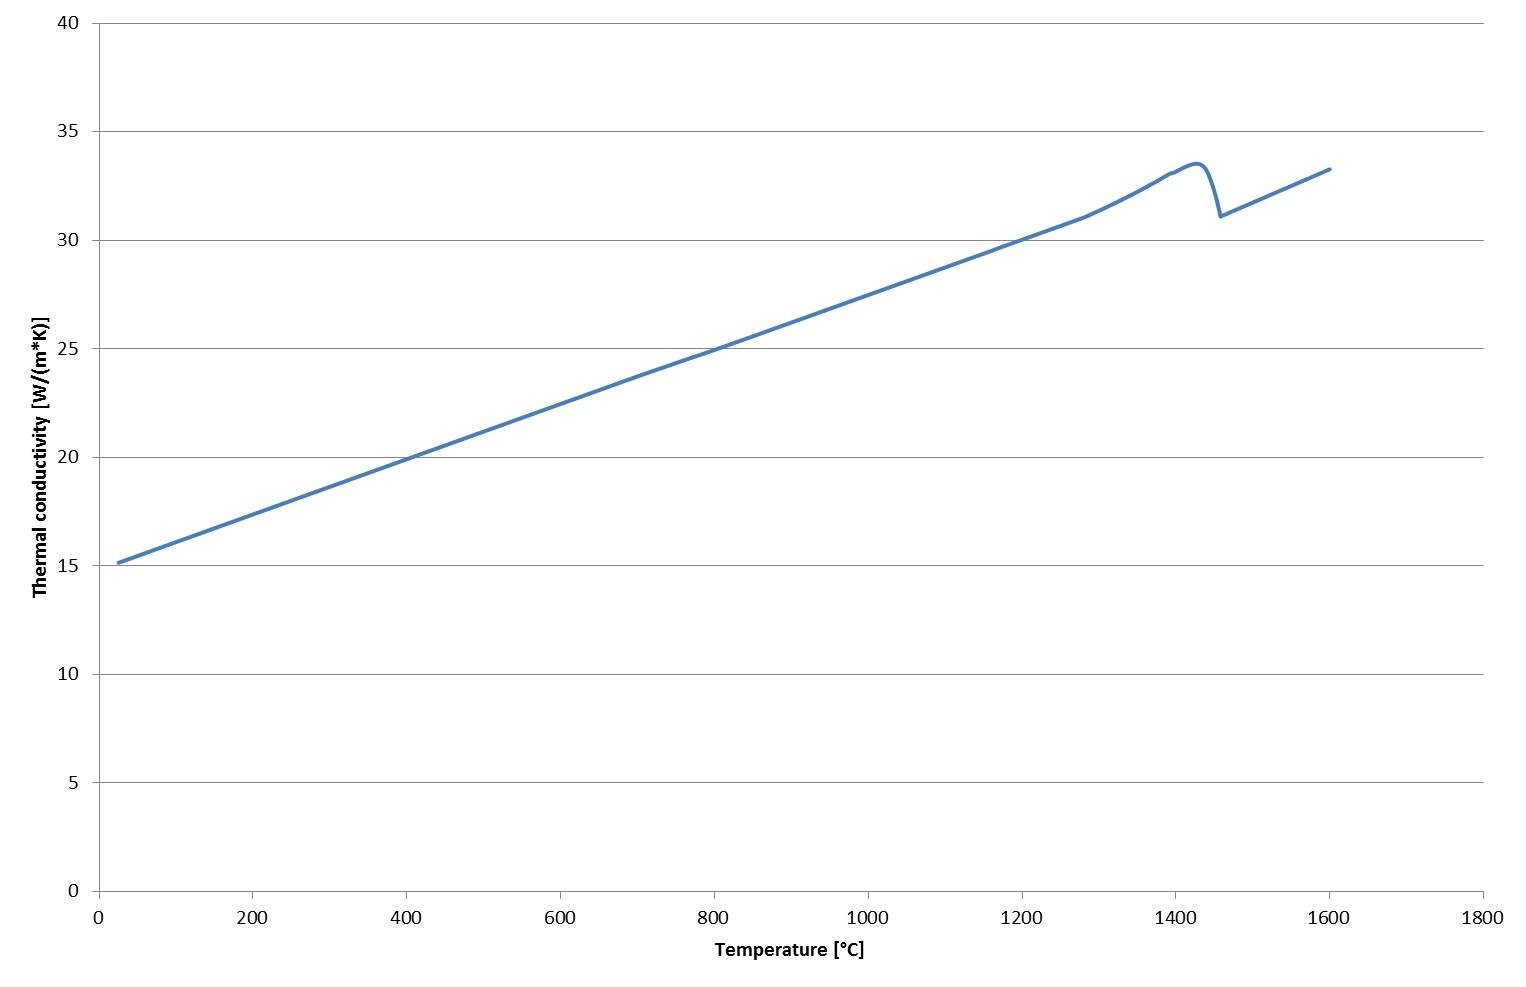
\includegraphics[width=0.8\textwidth]{images/thermalconductivity}
 \caption{Thermal conductivity of 1.4301}
 \label{img:thermalconductivity}
\end{figure}

\begin{figure}[htbp]
 \centering
 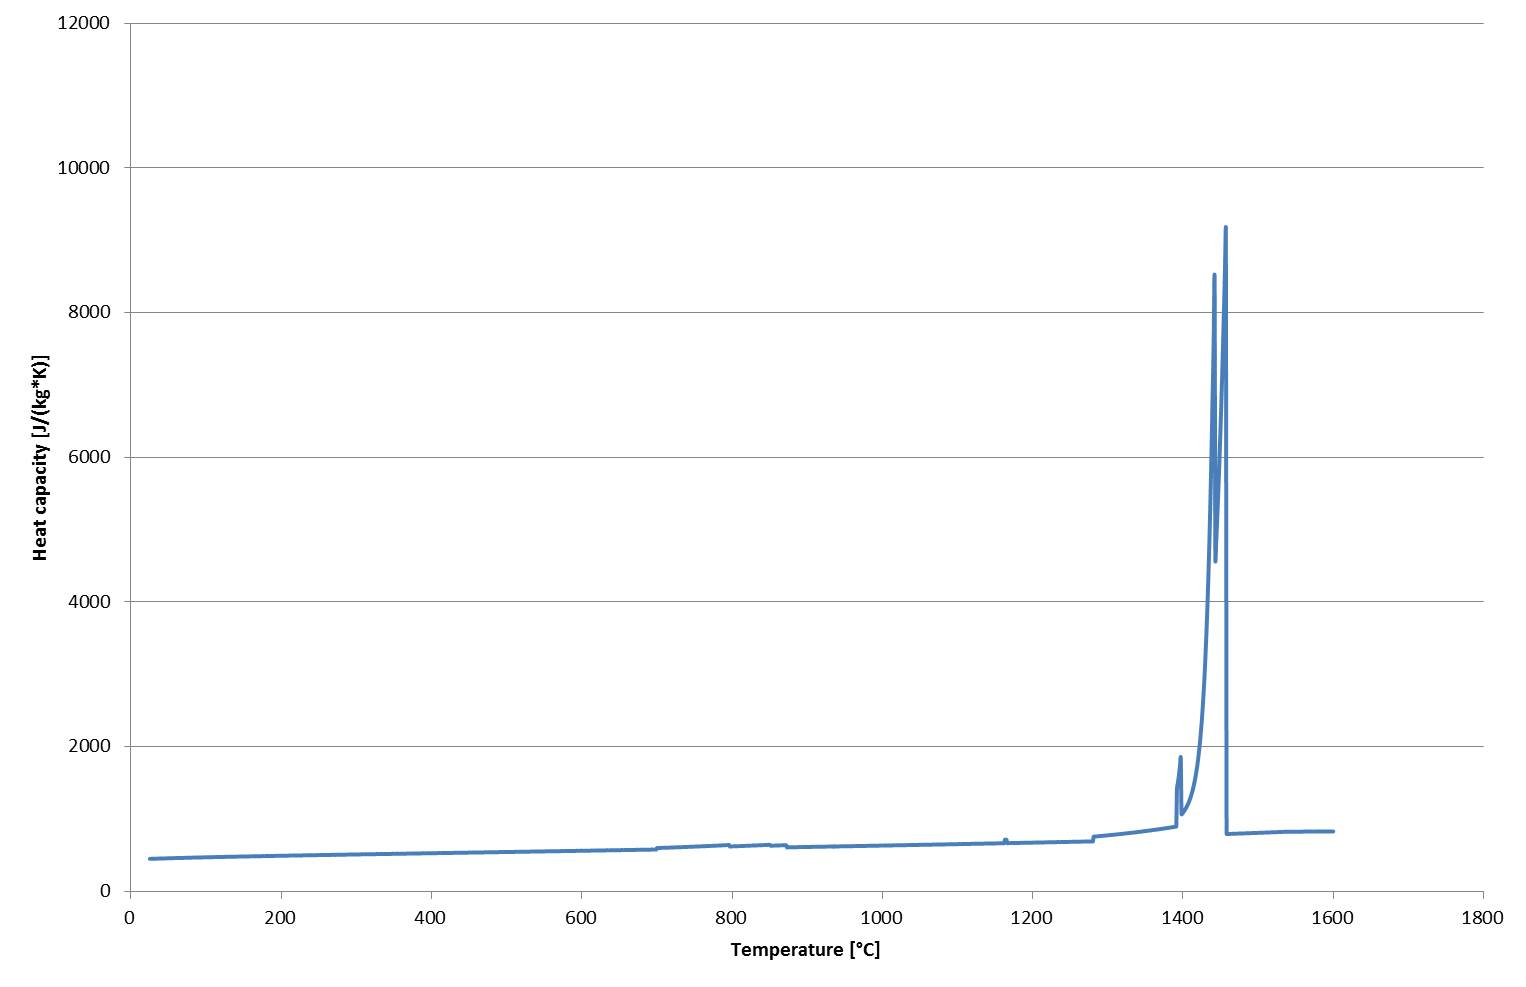
\includegraphics[width=0.8\textwidth]{images/heatcapacity}
 \caption{Heat capacity of 1.4301}
 \label{img:heatcapacity}
\end{figure}

\begin{figure}[htbp]
 \centering
 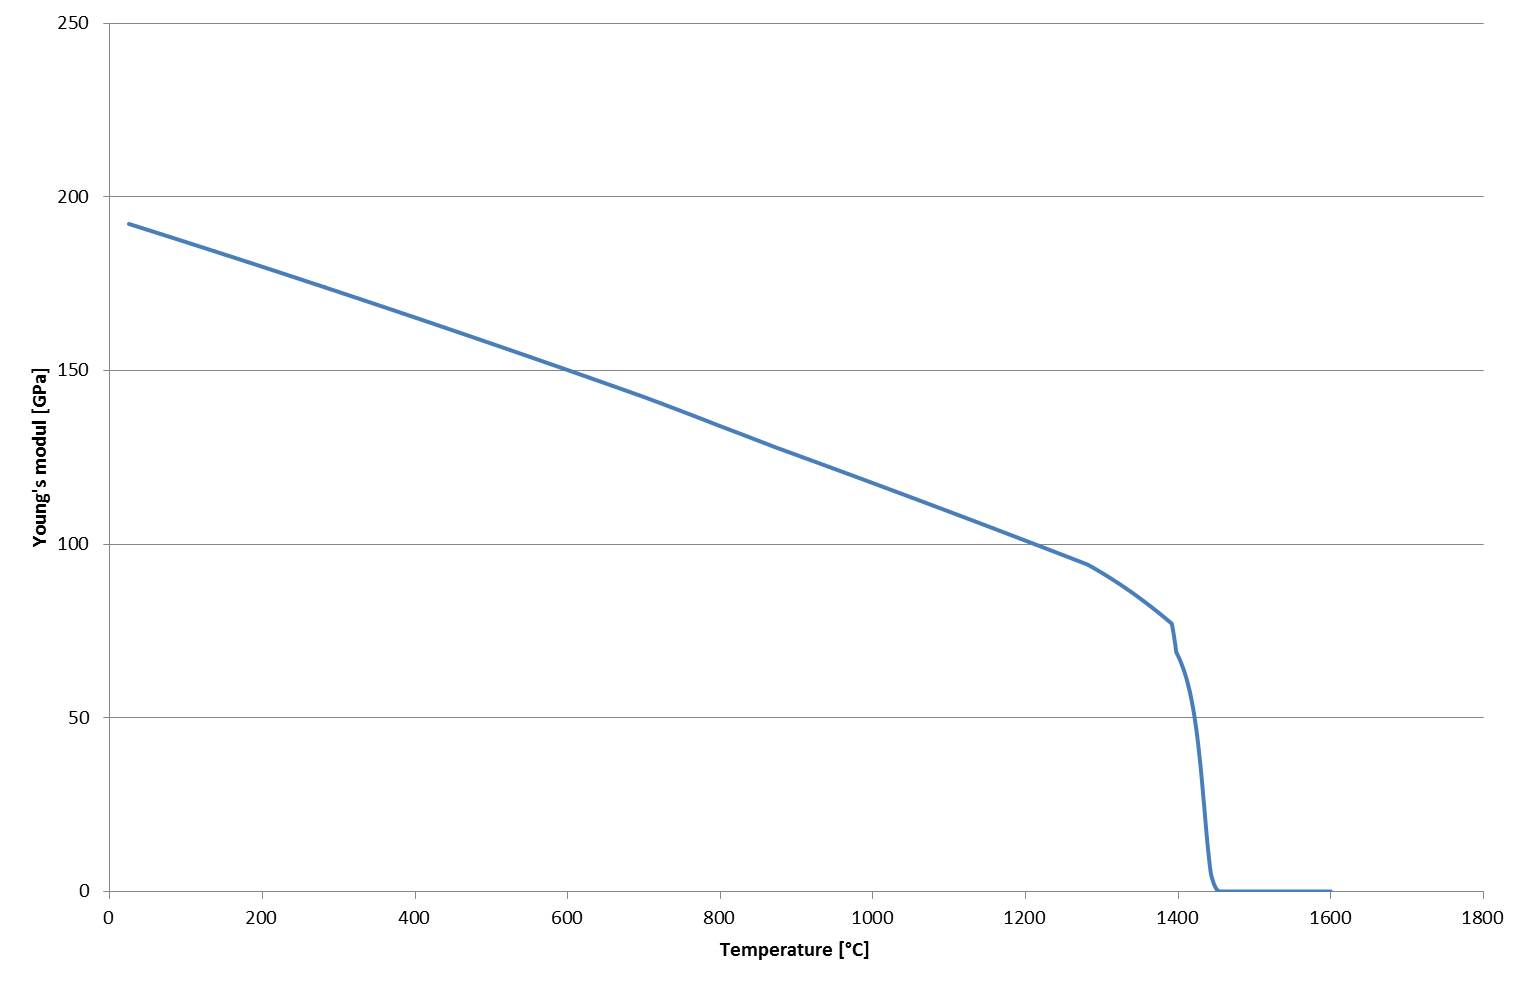
\includegraphics[width=0.8\textwidth]{images/youngsmodul}
 \caption{Young's modul of 1.4301}
 \label{img:youngsmodul}
\end{figure}

It is necessary that the data describes the whole temperature range of the process. Further parameters are set constant and are pictured in \ref{table:processparameter}. 

\begin{table}[htbp]%[width=0.8\textwidth]
 \centering
 \caption{Constant process parameters (reference temperature 20°C)}
 \begin{tabular}{|c|c|c|}
 \hline
 Poison&0,3&-\\
 \hline
 Thermal expansion&0,000012&[1/K]\\
 \hline
 Emissivity&0,7&-\\
 \hline
 Heat transfer coeff.&4,5&[W/(m²K)]\\
 \hline
 Friction coeff.&0,4&-\\
 \hline
 Dissipation&0,9&\%\\
 \hline
 \end{tabular}
 \label{table:processparameter}
\end{table}

\subsection{Forging plan (ForgeBase)}
The settings of the forging simulation are based on the calculation of the forging software ForgeBase \ref{table:forgingplan}. The simulations are done for a four passes process on a block (workpiece - WP) with the dimensions of 150mm in height as well as in width and 600mm in length. However, only 400mm of the length are forged. The rest is provided for the manipulator to hold and move the WP. The WP is set as a plastic solid and is meshed with a brick mesh with 12544 elements. The upper and lower dies are set as rigid object. The manipulator is set up as a spring with a stiffness of 175 N/mm and the maximum clamping force of 222,4 kN.\par 

The passes in the simulation vary in height reduction and bite ratio. Between the passes the WP is rotated in positive and negative direction with 90° rotation angle. There are two models of movement. On the one hand the bottom die is fixed, though the top die moves with a speed of 80mm/s (Simufact). On the other hand the top and the bottom die move with a speed of 40mm/s (DEFORM; PEP/LARSTRAN).

\begin{figure}[htbp]
 \centering
 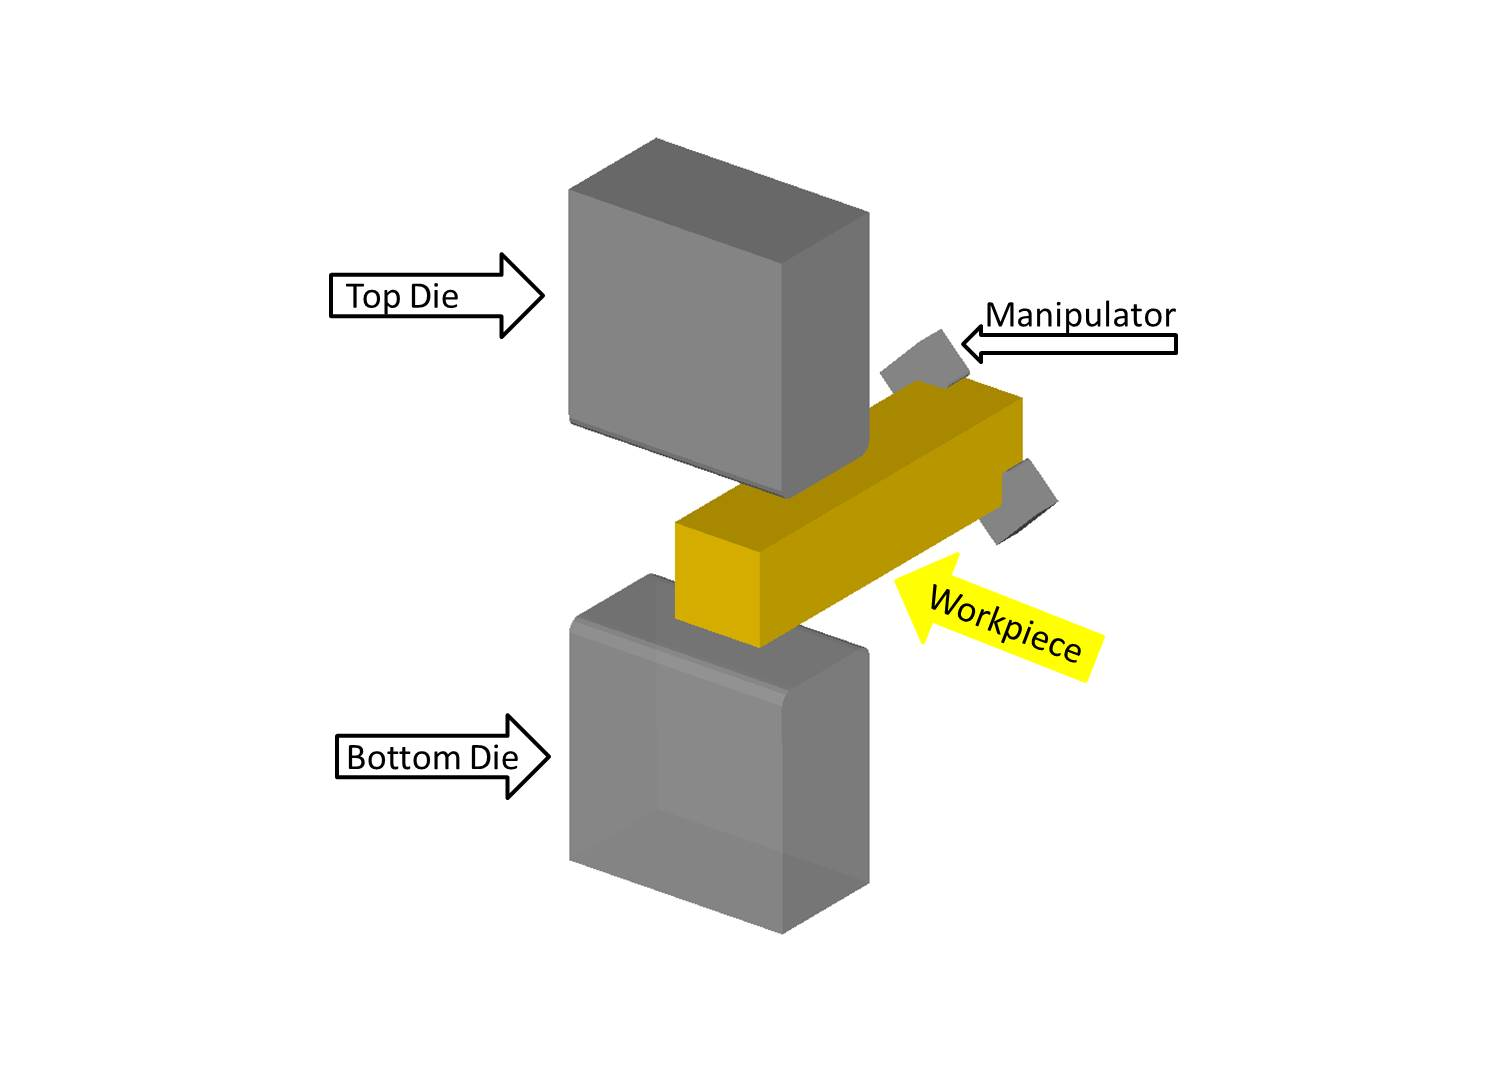
\includegraphics[width=0.8\textwidth]{images/processsetup}
 \caption{Illustration of the process setup from DEFORM}
 \label{img:processsetup}
\end{figure}

\begin{table}[htbp]%[width=1\textwidth]
 \footnotesize
 \centering
 \caption{Forging plan from ForgeBase}
 \begin{tabular}{|c|c|c|c|c|c|c|c|}
 \hline
 Pass Nr.&Reduction&Height 1&Width 1&Height 2&Width 2&Rotation&Bite width\\
 & [mm] & [mm] & [mm] & [mm] & [mm] & [$^{\circ}$] & [mm]\\
 \hline
 0&0&150&150&150&150&0&0\\
 \hline
 1&28&122&162&122&162&0&105\\
 \hline
 2&30&132&132&132&132&90&85\\
 \hline
 3&25&107&143&107&143&-90&92\\
 \hline
 4&27&116&116&116&116&90&75\\
 \hline
 \end{tabular}
 \label{table:forgingplan}
\end{table}

Moreover, the heat treatment before and during the process is of great importance. Before the first pass starts, the WP gets heated up to 1200°C for 2 hours. It is vital, that the WP does have a homogeneous distribution. During the forging passes, heat is getting lost by the effects of emission and the heat transfers to the dies. Because of that, a second heat is necessary between the second and the third pass. The WP is heated up again to 1200°C within 1 hour. After the last pass the WP cools down upon air to room temperature.

\section{Previous work}

The described process has previously been investigated using Simufact.forming from simufact engineering gmbh. \textit{Zusammenfassung Ergebnisse Yuwei}

\include{material modelling}
\section{Validation}

For the modelling of the described process, different software packages are available. Specifically, DEFORM-3D from Scientific Forming Technologies Corporation,Columbus, USA, FORGE from Transvalor, Mougins, France, and a combination of PEP (Pre- and Postprocessing Environment for Programmers) developed at IBF and LARSTRAN from LASSO Ingenieurgesellschaft mbH, Leinfelden, Germany have been used. These packages differ in their ease of use and freedom in modelling. A comparison of both usability and results will be made here.

\subsection{DEFORM-3D}

\subsection{FORGE}

\subsection{PEP/LARSTRAN}

%\include{cadconcept}
\section{Summary}

\section{Outlook}

The results of microstucture modelling have shown that small strain rates result in large values for the dynamically recrystallized volume fraction. This effect is due to the limitations of using absolute thresholds for microstructural parameters. The models should be extended to give a more dynamic model which allows a bigger range of these paramenters.

Furthermore, a systematic approach to the comparison of various FEM packages with each other and with reality should involve, as a first step, the research of the capabilities of the involved packages and the development of an according model process. Also, an even more detailed process model should be set up, using the same time increments, mesh, boundary conditions etc.

Lastly, a validation of the results in a real process is necessary. This includes a validation of both the microstructural model with grain sizes measured during the process and the process parameters such as die forces and material temperature development.

%\appendix
%\include{usedsymbols}
\listoffigures
\newpage
\bibliographystyle{alphadin}
\bibliography{hauptseminar_hibbe_nick_2014}
\include{appendix}
\end{document}
